\lhead{\begin{tikzpicture}[remember picture, overlay]
    \node [anchor=100,inner sep=0] (imagenIZQUIERDA) at (current page header area.north){
\includegraphics[width=18cm]{img/Encabezado.PNG}};
    \end{tikzpicture}}
    \rhead{Ángeles-Hurtado}
    \rfoot{\begin{tikzpicture}[remember picture, overlay]
    \node [anchor=140,inner sep=0] (imagenDERECHA) at (current page footer area.south){
\includegraphics[width=18cm]{img/Foot.PNG}};
    \end{tikzpicture}}
    %----------------------------------------------------------------------------------------
    \lfoot{ \thepage}
    % \renewcommand{\labelenumi}{\alph{enumi}.)} 
    %----------------------------------------------------------------------------------------
    %----------------------------------------------------------------------------------------
    %	TITLE SECTION
    %----------------------------------------------------------------------------------------
    
    \setlength{\droptitle}{-5\baselineskip} % Move the title up
    \title{\textbf{Estudio de tiempos y movimientos en el ensamble de un circuito electrónico utilizando diferentes métodos para su optimización }} % Article title
    
     \author{ 
     \textsc{Zavala Gonzalez, Luis Alonso}\\ 
    %  Afiliación:
     \texttt{ Instituto Tecnológico de Querétaro } \\ 
     \texttt{ Tecnológico Nacional de México } \\ 
     \texttt{Querétaro, México}\\ 
     \texttt{l22140885@queretaro.tecnm.mx} 
     \and 
     \textsc{Ángeles-Hurtado, Luis Alberto}\\ 
    %  Afiliación:
     \texttt{ Instituto Tecnológico de Querétaro } \\ 
     \texttt{ Tecnológico Nacional de México } \\ 
     \texttt{Querétaro, México}\\ 
     \texttt{alb3rt0.ah@gmail.com} 
    }
    
    
    %----------------------------------------------------------------------------------------
    
    % \begin{document}
    
    % Print the title
    \maketitle
    \thispagestyle{fancy}
    
    %----------------------------------------------------------------------------------------
    %	ARTICLE CONTENTS
    %----------------------------------------------------------------------------------------
    
    % \section*{Resumen}
    % \textit{Palabras clave:}
    % El resumen (ancho de página) deberá contener entre 100 y 200 palabras tipo Adobe Devangari 11 puntos.
    
    \begin{abstract}
    \noindent 
    El resumen (ancho de página) deberá contener entre 100 y 200 palabras tipo Adobe Devangari 11 puntos.
    
    \end{abstract}
    % 
    % 
    \textbf{\textit{Palabras clave}}: {Tiempos, movimientos, análisis, muestreo, exacto, preciso.}
    % \keywords{First keyword should be the corresponding to the research area according with the authors guide. Maximum of 6 keywords.}
    
    \section{Introducción}
    
    % Define estudio de tiempos y movimientos
    % define que es ensamble
    % define que es circuito electronico
    % define el metodo de tiempos predeterminados
    % define optimización
    \begin{itemize}
        \item \textbf{{Estudio de tiempos y movimientos:}}
        Es el análisis de método, materiales, herramientas e instalación utilizada o que se ha de utilizar en la ejecución de un trabajo.
        \item \textbf{Ensamble:}
        Unir, juntar, ajustar, montar, encajar piezas en pocas palabras es la colocación de dos o más piezas para la conformación de un producto final.
        \item \textbf {Circuito electrónico:}
        Es un conjunto de elementos eléctricos conectados entre sí que permiten generar, transportar y utilizar la energía eléctrica con la finalidad de transformarla en otro tipo de energía.
        \item \textbf{Método de tiempos predeterminados:}
        Es una mejora, en pocas palabras se refiere a la capacidad de hacer o resolver alguna cosa de la manera más eficiente posible y, en el mejor de los casos, utilizando la menor cantidad de recursos.
        \item \textbf{Optimización:}
        Buscar la mejor manera de realizar una actividad.
        \end{itemize}
    % 
    % 
    \section{Justificación}
    
    %\begin{itemize}
    El estudio de tiempos y movimientos en el ensamble de circuitos electrónicos utilizando diferentes métodos de optimización es crucial para maximizar la eficiencia operativa, reducir costos y mejorar la calidad del producto. Al analizar detalladamente cada paso del proceso de ensamble, se pueden identificar oportunidades para eliminar desperdicios, minimizar tiempos de producción y mejorar el proceso. Esto no solo aumenta la productividad y la rentabilidad de la empresa, sino que también garantiza la satisfacción del cliente al ofrecer productos de alta calidad en tiempos más rápidos.
        
    %\end{itemize}
    % 
    % 
    \section{Descripción del problema}
    \begin{itemize}
        \item Se debe describir la desviación o diferencia del ``es'' con respecto al ``debe ser''.
        \item Se debe hacer alusión a la incógnita científica*.
        \item Debe de tener Referencias científicas, URL, tesis, etc.
    \end{itemize}
    
    \textbf{*La incógnita científica es el elemento cuya solución incrementa el conocimiento científico.}
    % 
    % 
    \section{Fundamentación teórica}
    
    Es la parte medular y de mayor discusión, deberá ser la fundamentación de la hipótesis, por tanto se deberá señalar claramente la razón de la suposición y fundamentación de la misma. Únicamente referencias científicas.
    \begin{itemize}
        \item Se debe de retomar el tema que se planteo en la introducción, pero ahora profundizando para clarificar la incógnita científica y se pueda plantear la hipótesis.
        \item Se debe de retomar la descripción del problema, pero ahora a profundidad del (los) objeto(s) de estudio. 
        \item Se debe de profundizar en las metodologías que se ha usado para el estudio del tema.
        \item Referencias solo de artículos y libros científicos.
    \end{itemize}
    % 
    % 
    \section{Hipótesis}
    
    Es la suposición con fundamento científico relativa a la solución del problema, necesidad o de cómo se aprovecha la oportunidad con la incógnita científica y se fundamenta con: 1. Una suposición (en afirmativo o negativo) y ésta deberá vincularse con:
    2. La fundamentación científica que deberá ser precisa 3. Una entidad de comparación para probar la suposición y
    4. La variable con que se califica o cuantifica la comparación o se prueba la hipótesis.
    
    \begin{itemize}
        \item Se debe de identificar claramente la suposición científica
        \item Se debe de identificar claramente el fundamento científico
        \item Se debe identificar claramente la variable de respuesta
        \item Se debe identifican claramente las realidades o modelos contrastantes
        \item Se debe de establecer las variables asociadas, explicativas o que tienen relación funcional con la variable de respuesta
    \end{itemize}
    % 
    % 
    \section{Objetivo}Reducir el tiempo total de ensamble del circuito electrónico en un 10 por ciento mediante la aplicación de técnicas de optimización de procesos.
    \begin{itemize}
        \item Se debe establecer que se pretende probar la hipótesis
    \end{itemize}
    
    \subsection{Objetivos específicos }
    
    \begin{itemize}
        \item Medir el tiempo requerido para cada etapa del ensamble del circuito electrónico.
        \item Analizar las áreas de ineficiencia en el proceso de ensamble.
        \item Investigar y proponer mejoras en el diseño del circuito electrónico para facilitar su ensamble, reducir la complejidad y el número de pasos requeridos.
        \item Capacitar al personal en los nuevos métodos y procedimientos de ensamble optimizados.
        \item Establecer un sistema de retroalimentación continua para recopilar sugerencias e ideas de mejora del personal involucrado en el proceso de ensamble.
    
    \end{itemize}
    
    % 
    % 
    \section{Cuerpo (Metodología, modelo matemático, etc.)}
    
        \textbf{Preparación de materiales}: Verificar que todos los componentes necesarios estén disponibles y en buenas condiciones para su uso. \ref{anexo:listaMateriales}.
    
        \textbf{Bosquejo de Distribución}: Asegurar que el espacio de trabajo esta limpio y en aptas condiciones, ordenar todos los materiales como se muestra en el bosquejo para su mejor organización y una búsqueda mas fácil de los mismos. \ref{anexo:bosquejo}.
    
        \textbf{Manual de ensamblaje}: Seguir el Manual de ensamblaje del ESP32-C6 para instalar correctamente los componentes y realizar la prueba. \ref{anexo:manual}.
    
    
    \begin{itemize}
        \item Se debe establecer que se habrá de hacer, como, conque, y donde para obtener la información que permita probar la hipótesis.  
        \item Se debe desglosar de acuerdo a los objetivos específicos. 
        \item Se debe establecer una estrategia metodológica por cada objetivo específico. De manera simplista se podría decir que se cambia el verbo en infinitivo por su respectivo adverbio.
        \item En cada objetivo se debe describir que método, que materiales y que equipo se usará para conseguirlo.
        \item Se deben tener referencias Figura %\ref{fig:lcd-16x2}.%
    \end{itemize}
    % 
    
    % 
    \subsection{Prepara tu documento}
    
    Antes de que comiences a utilizar esta plantilla, es recomendable que prepare la información que contendrá en un archivo aparte. 
    Ten preparadas tus gráficas, así como también las tablas aparte, para que sea más fácil integrarlo. 
    Se recomienda fuertemente el uso de \textbf{formato Enhanced Metafile (.emf) para imágenes y gráficas} de resolución óptima. 
    Finalmente, completa y organiza el contenido antes de darle el formato de esta plantilla. 
    
    \subsection{Acrónimos y Abreviaciones}
    
    Los acrónimos y abreviaciones deberán ser definidos únicamente la primera vez que aparecen en el texto, esto para que el lector entienda lo que significan.
    
    \subsection{Ecuaciones}
    
    Las ecuaciones son una excepción a las especificaciones prescritas de esta plantilla. 
    Deberá determinar si su ecuación debe escribirse o no utilizando la fuente Adobe Devangari. 
    Para crear ecuaciones multinivel, puede ser necesario tratar la ecuación como un gráfico e insertarla en el texto después de aplicar el estilo de la platilla.
    Las ecuaciones serán enumeradas de manera consecutiva, y el número de ecuación, entre paréntesis, se colocan al ras de la derecha, utilizando una tabulación derecha. 
    
    \begin{equation}
        \label{eq1}
        x + y = z 
    \end{equation}
    
    Es importante asegurarse de que los símbolos de la ecuación sean definidos antes o inmediatamente después de la ecuación. Utilice “(1)”, en vez de “Eq. 1” al enumerar las ecuaciones, excepto al principio de una oración: “La ecuación (\ref{eq1}) es…”
    
    \section{Resultados y discusión}
    
    
    
    Operador: Cristian Jonathan Morales Piña
    
    
    
    \begin{figure}
        \centering
        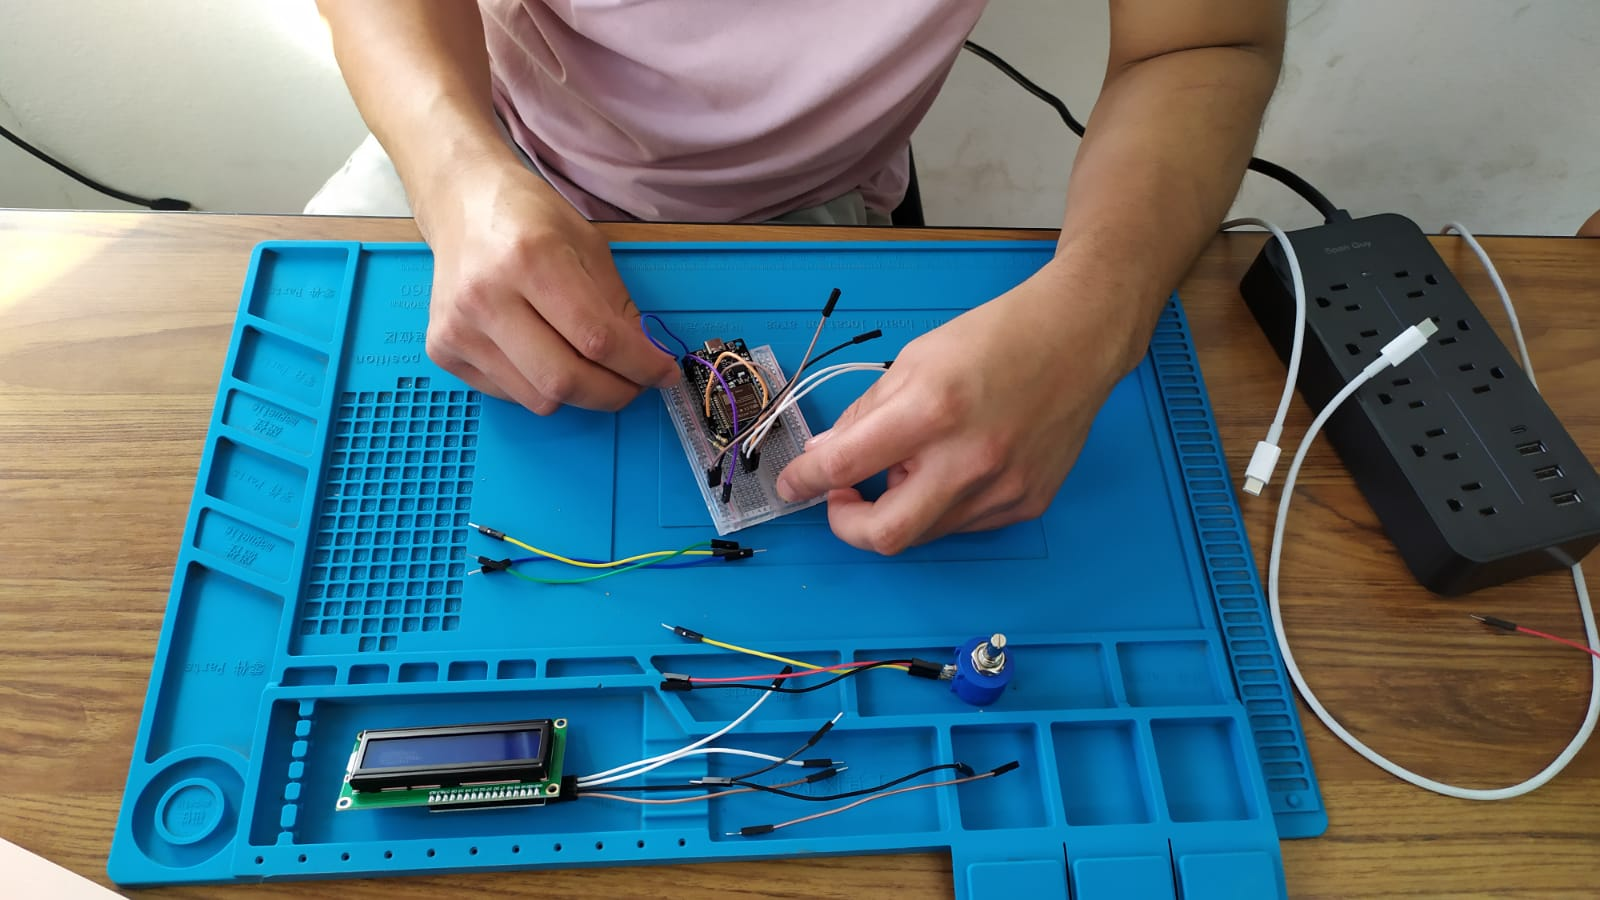
\includegraphics[trim = {60mm 40mm 80mm 60mm},clip,scale=0.2]{35/Img/ensamble1.jpeg}
        \caption{Evidencia 1}
        \label{Evidencia 1}
    \end{figure}
    
    \begin{figure}
        \centering
        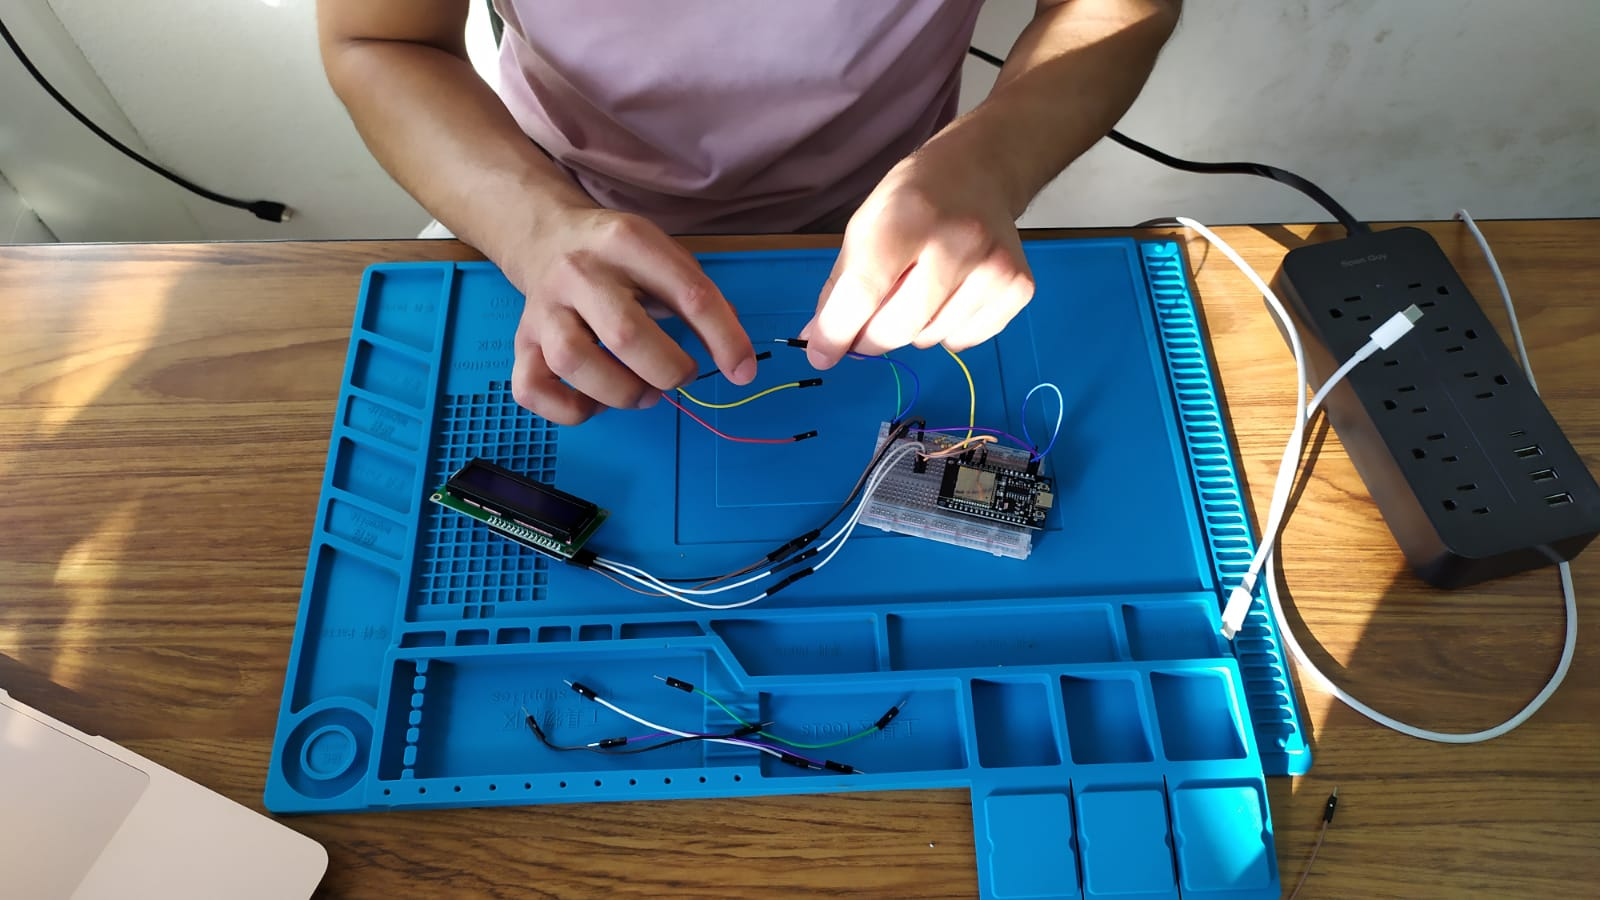
\includegraphics[trim = {65mm 40mm 80mm 60mm},clip,scale=0.2]{35/Img/ensamble2.jpeg}
        \caption{Evidencia 2}
        \label{Evidencia 2}
    \end{figure}
    
    \begin{figure}
        \centering
        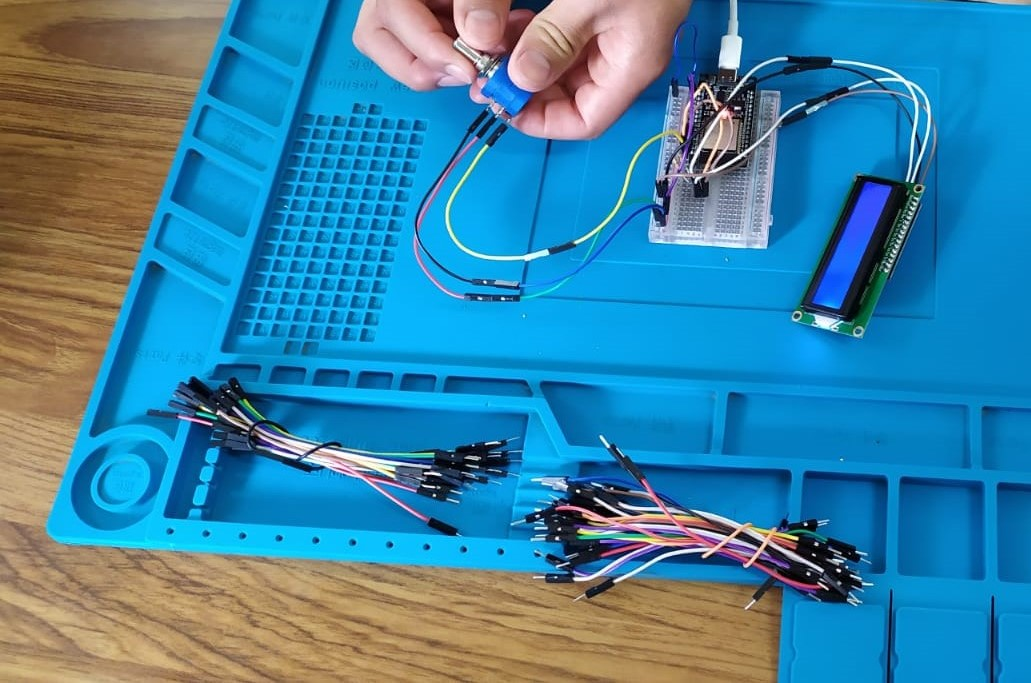
\includegraphics[trim = {65mm 40mm 80mm 60mm},clip,scale=0.6]{35/Img/ensamble3.jpeg}
        \caption{Evidencia 3}
        \label{Evidencia 3}
    \end{figure}
    
    \begin{figure}
        \centering
        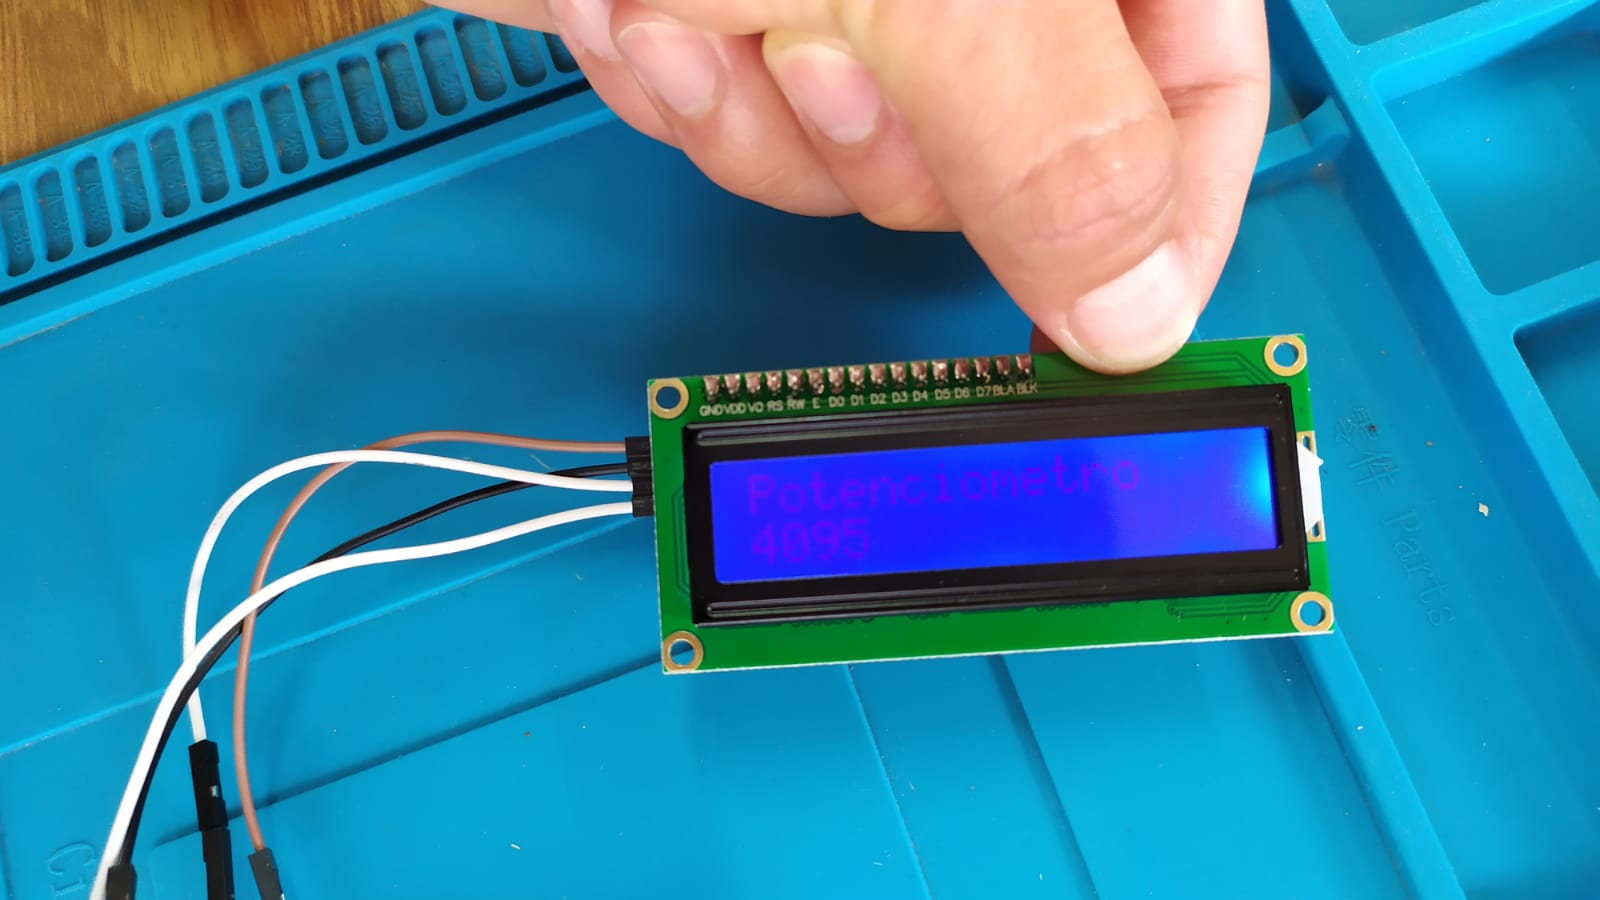
\includegraphics[trim = {65mm 40mm 80mm 60mm},clip,scale=0.2]{35/Img/ensamble4.jpeg}
        \caption{Evidencia 4}
        \label{Evidencia 4}
    \end{figure}
    
    
    
    \subsection{Autores y Afiliaciones}
    
    Para distinguir las afiliaciones de los autores, utilice superíndices iniciando con el número 1, 2, etc., sucesivamente, esto dependerá de la cantidad de los departamentos a los que estén afiliados los autores. En caso de que todos los autores pertenezcan a una mismo departamento e institución, utilizar sólo el superíndice 1. 
    
    \subsection{Identificar los encabezados}
    
    Se les recuerda a los autores que los encabezados deben de estar conforme los solicita la guía del autor. De ahí se puede adaptar el trabajo para que sea más fácil de entender para el lector.
    Los encabezados organizan los temas sobre una base relacional y jerárquica. Por ejemplo, el título del documento es encabezado del texto principal porque todo el material posterior se relaciona y elabora sobre este tema. 
    
    \subsection{Tablas y Figuras}
    
    \begin{enumerate}
        \item Posición de las tablas y figuras: Coloque las figuras y las tablas en la parte superior e inferior de las columnas. Evite colocarlos en medio. Las figuras y las tablas grandes pueden abarcar ambas columnas. Los títulos de las figuras deben de estar debajo de las mismas; los títulos de las tablas deben aparecer encima de ellas. Insértese las figuras y los cuadros después de citarse en el texto. Utilice la abreviatura “Fig. 1”, incluso al principio de una oración. 
    \end{enumerate}
    
    \section{Conclusiones}
    
    Se describe aquí el alcance del trabajo, logros obtenidos y perspectivas para el futuro de este. Se sugiere colocar información cuantitativa obtenida.
    
    \section{Agradecimientos}
    
    Es importante darles su debido reconocimiento a los laboratorios, instituciones, organizaciones, entre otros que han sido participes para la culminación de este trabajo. También es importante mencionar, fondos, proyectos, becas, entre otros que se le han otorgado al o los autores para realizar el trabajo de investigación. Ejemplo: “Los autores agradecen al Concejo Nacional de Ciencia y Tecnología por los recursos otorgados…”
    
    \section*{Referencias}
    
    % Ejemplo
    %  @Article{article,
    % 	author = "Author1 LastName1 and Author2 LastName2 and Author3 LastName3",
    % 	title = "Article Title",
    % 	volume = "30",
    % 	number = "30",
    % 	pages = "10127-10134",
    % 	year = "2013",
    % 	doi = "10.3389/fnins.2013.12345",
    % 	URL = "http://www.frontiersin.org/Journal/10.3389/fnins.2013.12345/abstract",
    % 	journal = "Frontiers in Neuroscience"
    % }
    
    % @book{book,
    %   author    = {Author Name}, 
    %   title     = {The title of the work},
    %   publisher = {The name of the publisher},
    %   address   = {The city},
    %   year      = 1993,
    % }
    
    % @incollection{chapter,
    %   author       = {Bauthor Surname}, 
    %   title        = {The title of the work},
    %   editor       = {Editor Name},
    %   booktitle    = {The title of the book},
    %   publisher    = {The name of the publisher},
    %   address      = {The city},
    %   year         = 2002,
    %   pages        = {201-213},
    % }
    
    % @InProceedings{conference,
    %   author = {Cauthor Name and Dauthor Surname and Fauthor LastName},
    %   title = {The title of the work},
    %   booktitle = {The title of the conference proceedings},
    %   year = 1996,
    %   publisher = {The name of the publisher},
    %   editor = {Editor Name1 and Editor Name2},
    %   pages = {41-50},
    % }
    
    % @book{cho,
    %   author       = {Gauthor Name1}, 
    %   title        = {The title of the work},
    %   publisher = {Country code and patent number},
    %   address      = {Patent Country},
    %   year = 2013
    % }
    
    % @book{patent,
    %   author    = {Hauthor Surname1}, 
    %   title     = {The title of the work},
    %   publisher = {Patent number},
    %   address   = {Patent country},
    %   year      = 2010,
    % }
    
    % % please use misc for datasets
    % @misc{dataset, 
    % 	author = "Author1 LastName1 and Author2 LastName2 and Author3 LastName3",
    % 	title = "Data Title",
    % 	year = "2011",
    % 	doi = "10.000/55555",
    % 	URL = "http://www.frontiersin.org/",
    % }
    
    \bibliographystyle{ieeetr}
    \bibliography{35/referencias}
    % 
    % 
    %%%%%%%%%%%%%%%%%%%%%%%%%%%%%%%%%%
    \appendix
    %%%%%%%%%%%%%%%%%%%%%%%%%%%%%%%%%%
    % 
    % 
    \newpage
    
    \centering{\section[\appendixautorefname{}]{Apéndice}}\label{anexo:bosquejo}
    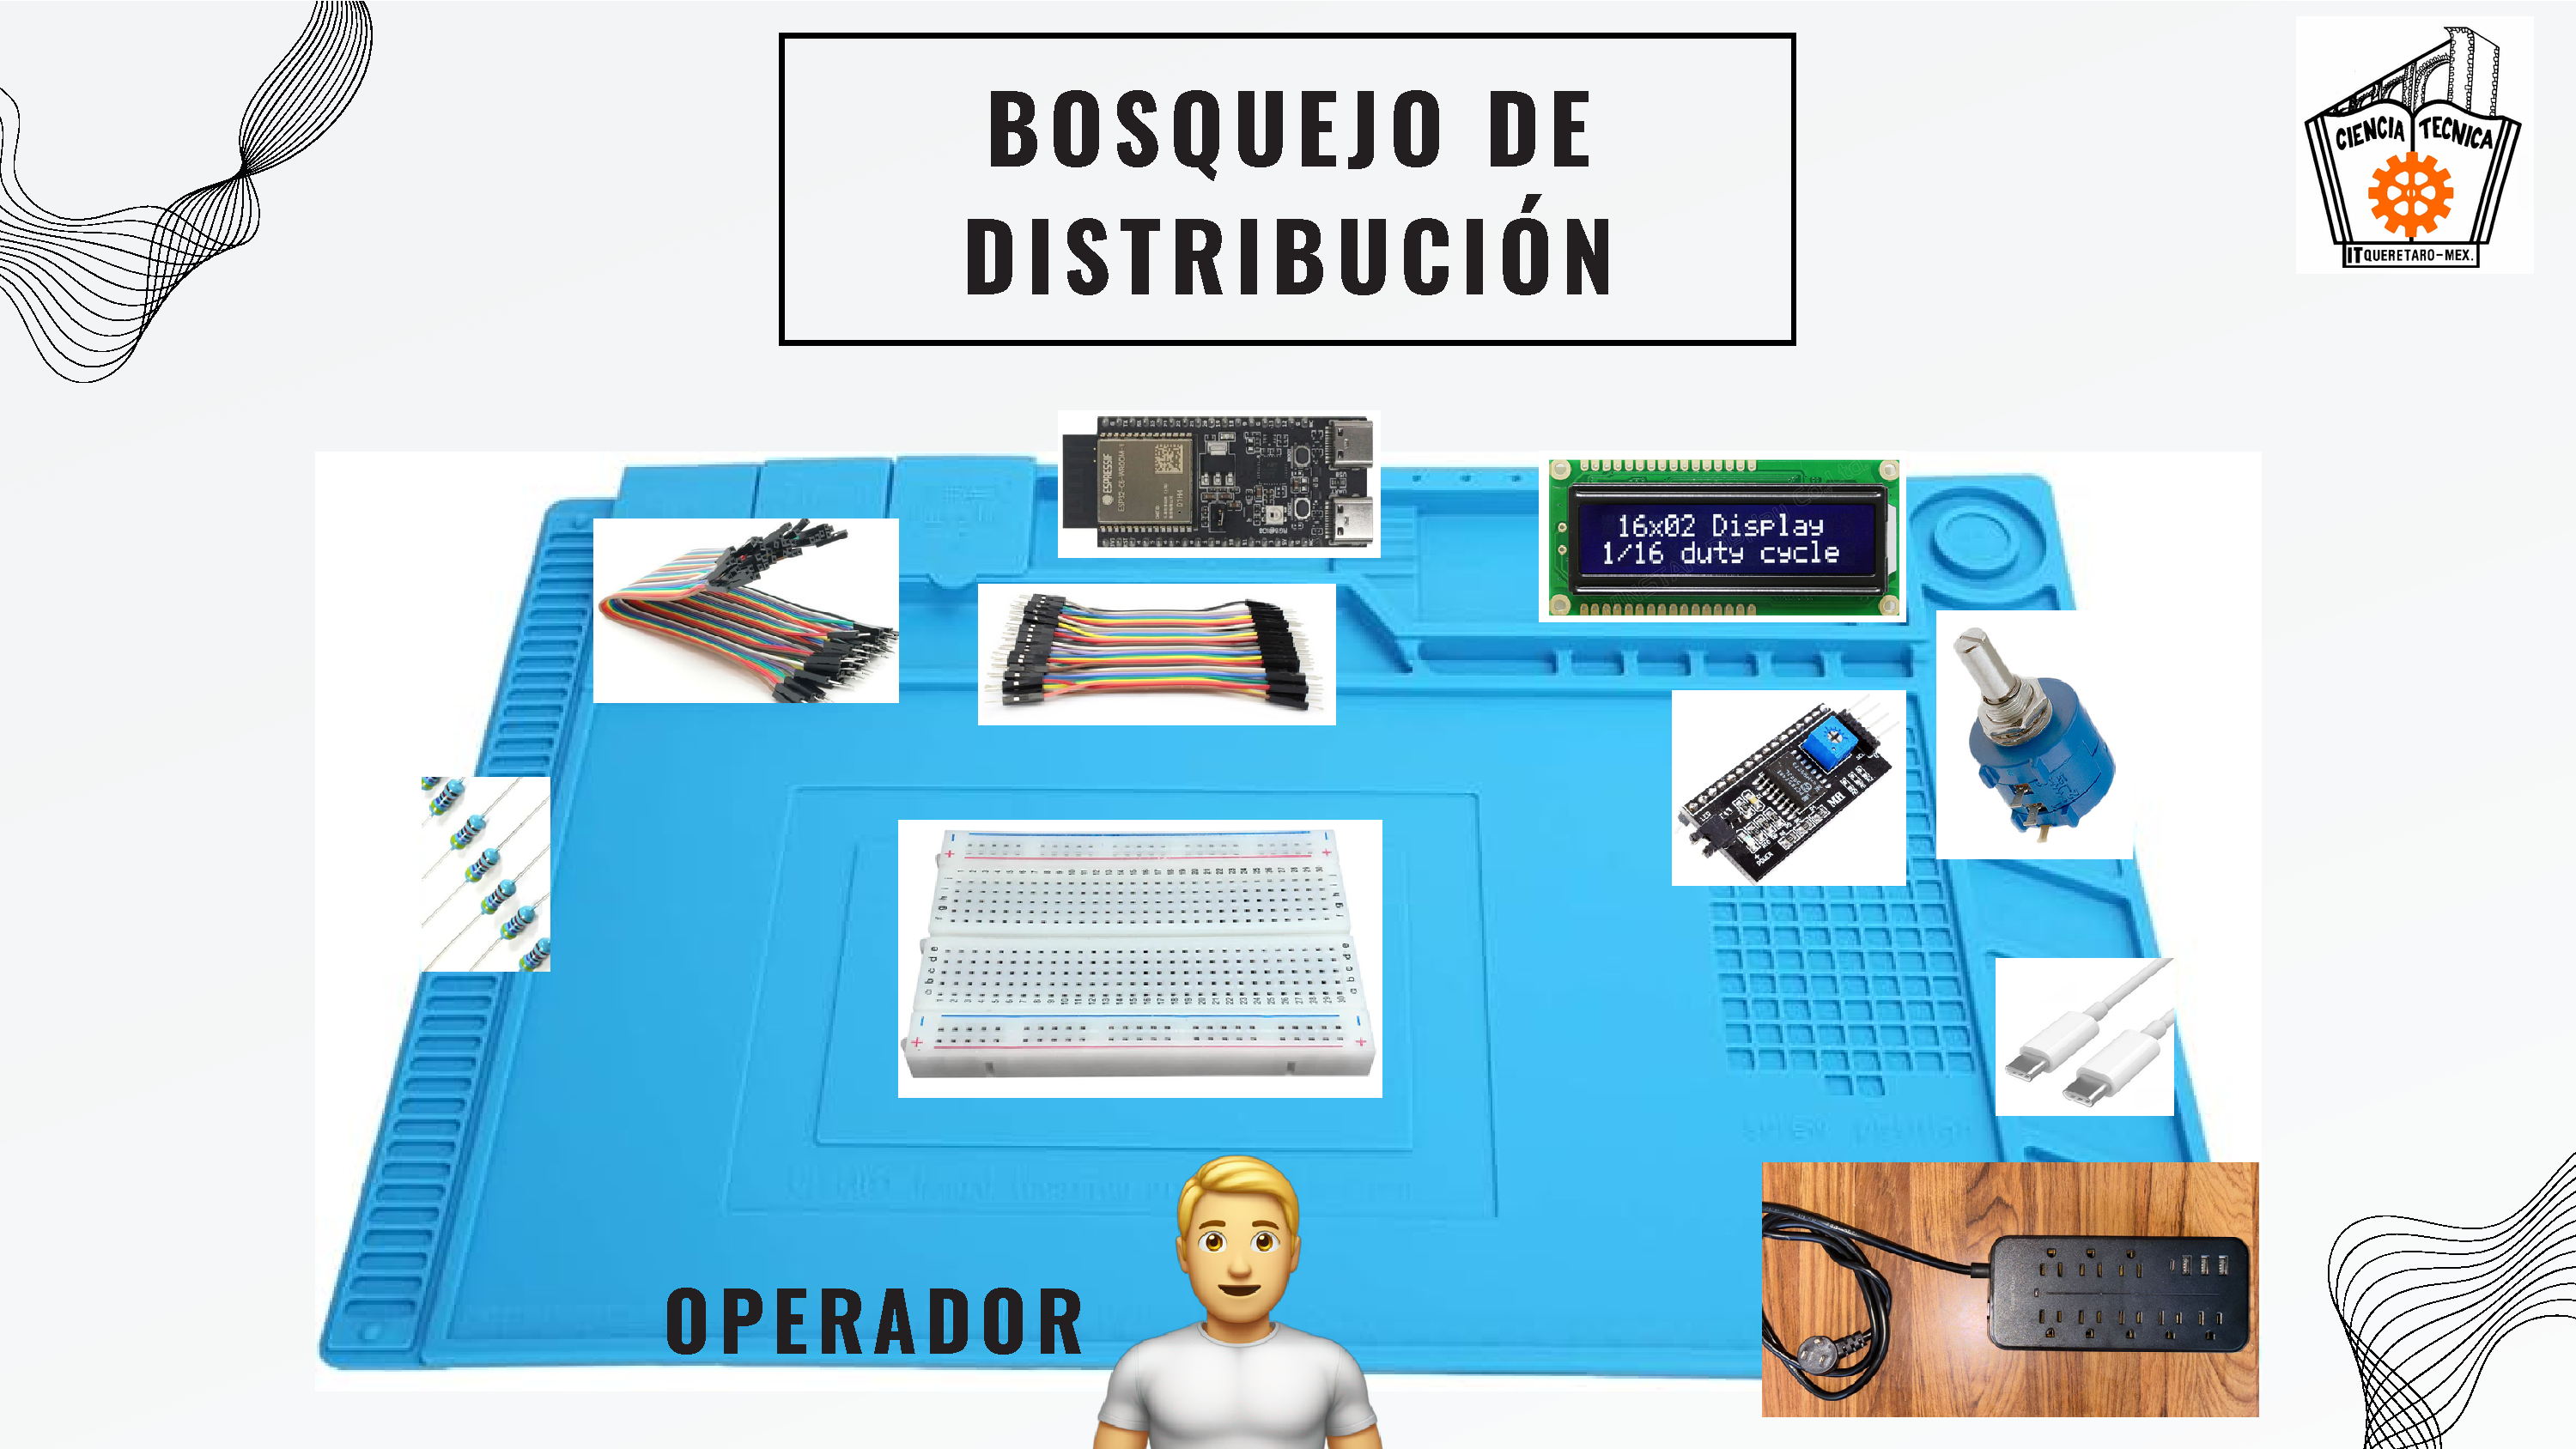
\includepdf[pages=-]{35/Img/bosquejoDistribucion.pdf}
    
    
    
    
    \centering{\section[\appendixautorefname{}]{Apéndice}}\label{anexo:listaMateriales}
    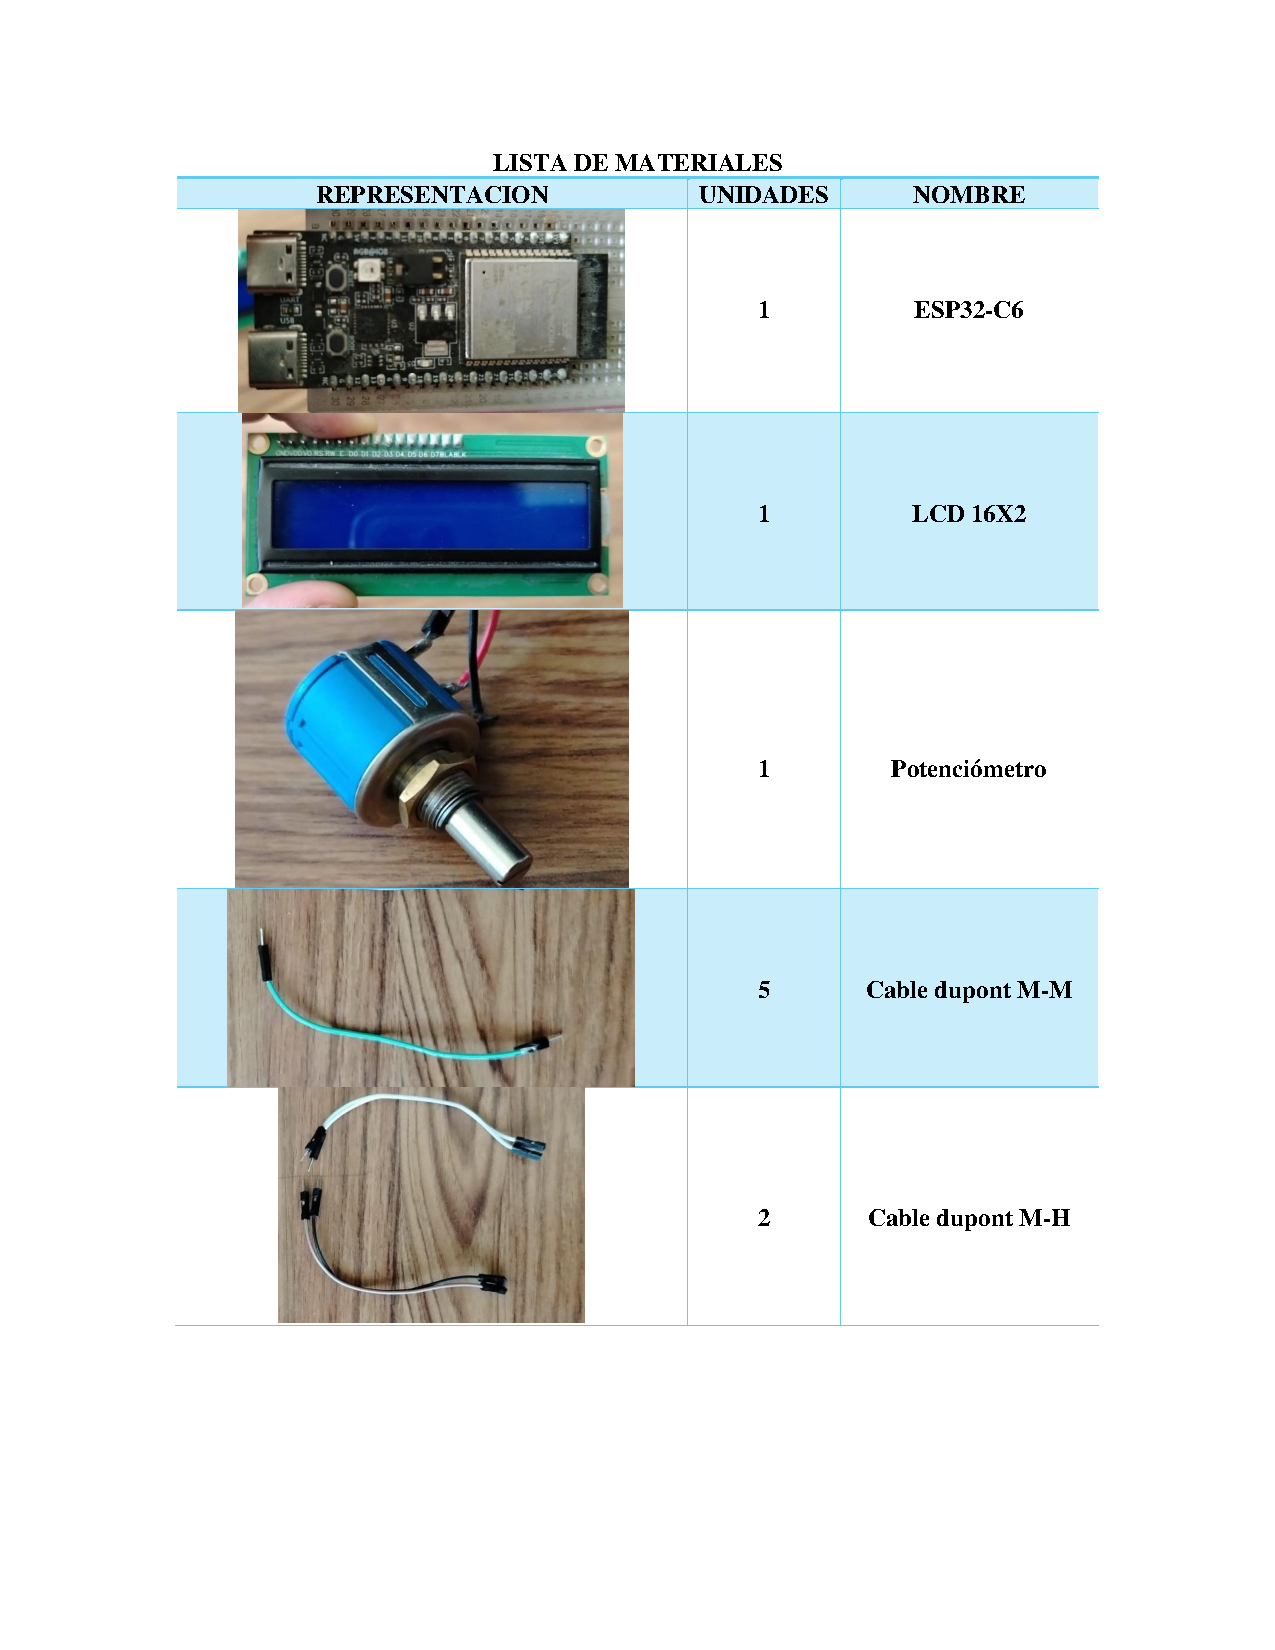
\includepdf[pages=-]{35/Img/listaMateriales.pdf}
    
    
    %%%
    \centering{\section[\appendixautorefname{}]{Apéndice}}\label{anexo:resultados}
    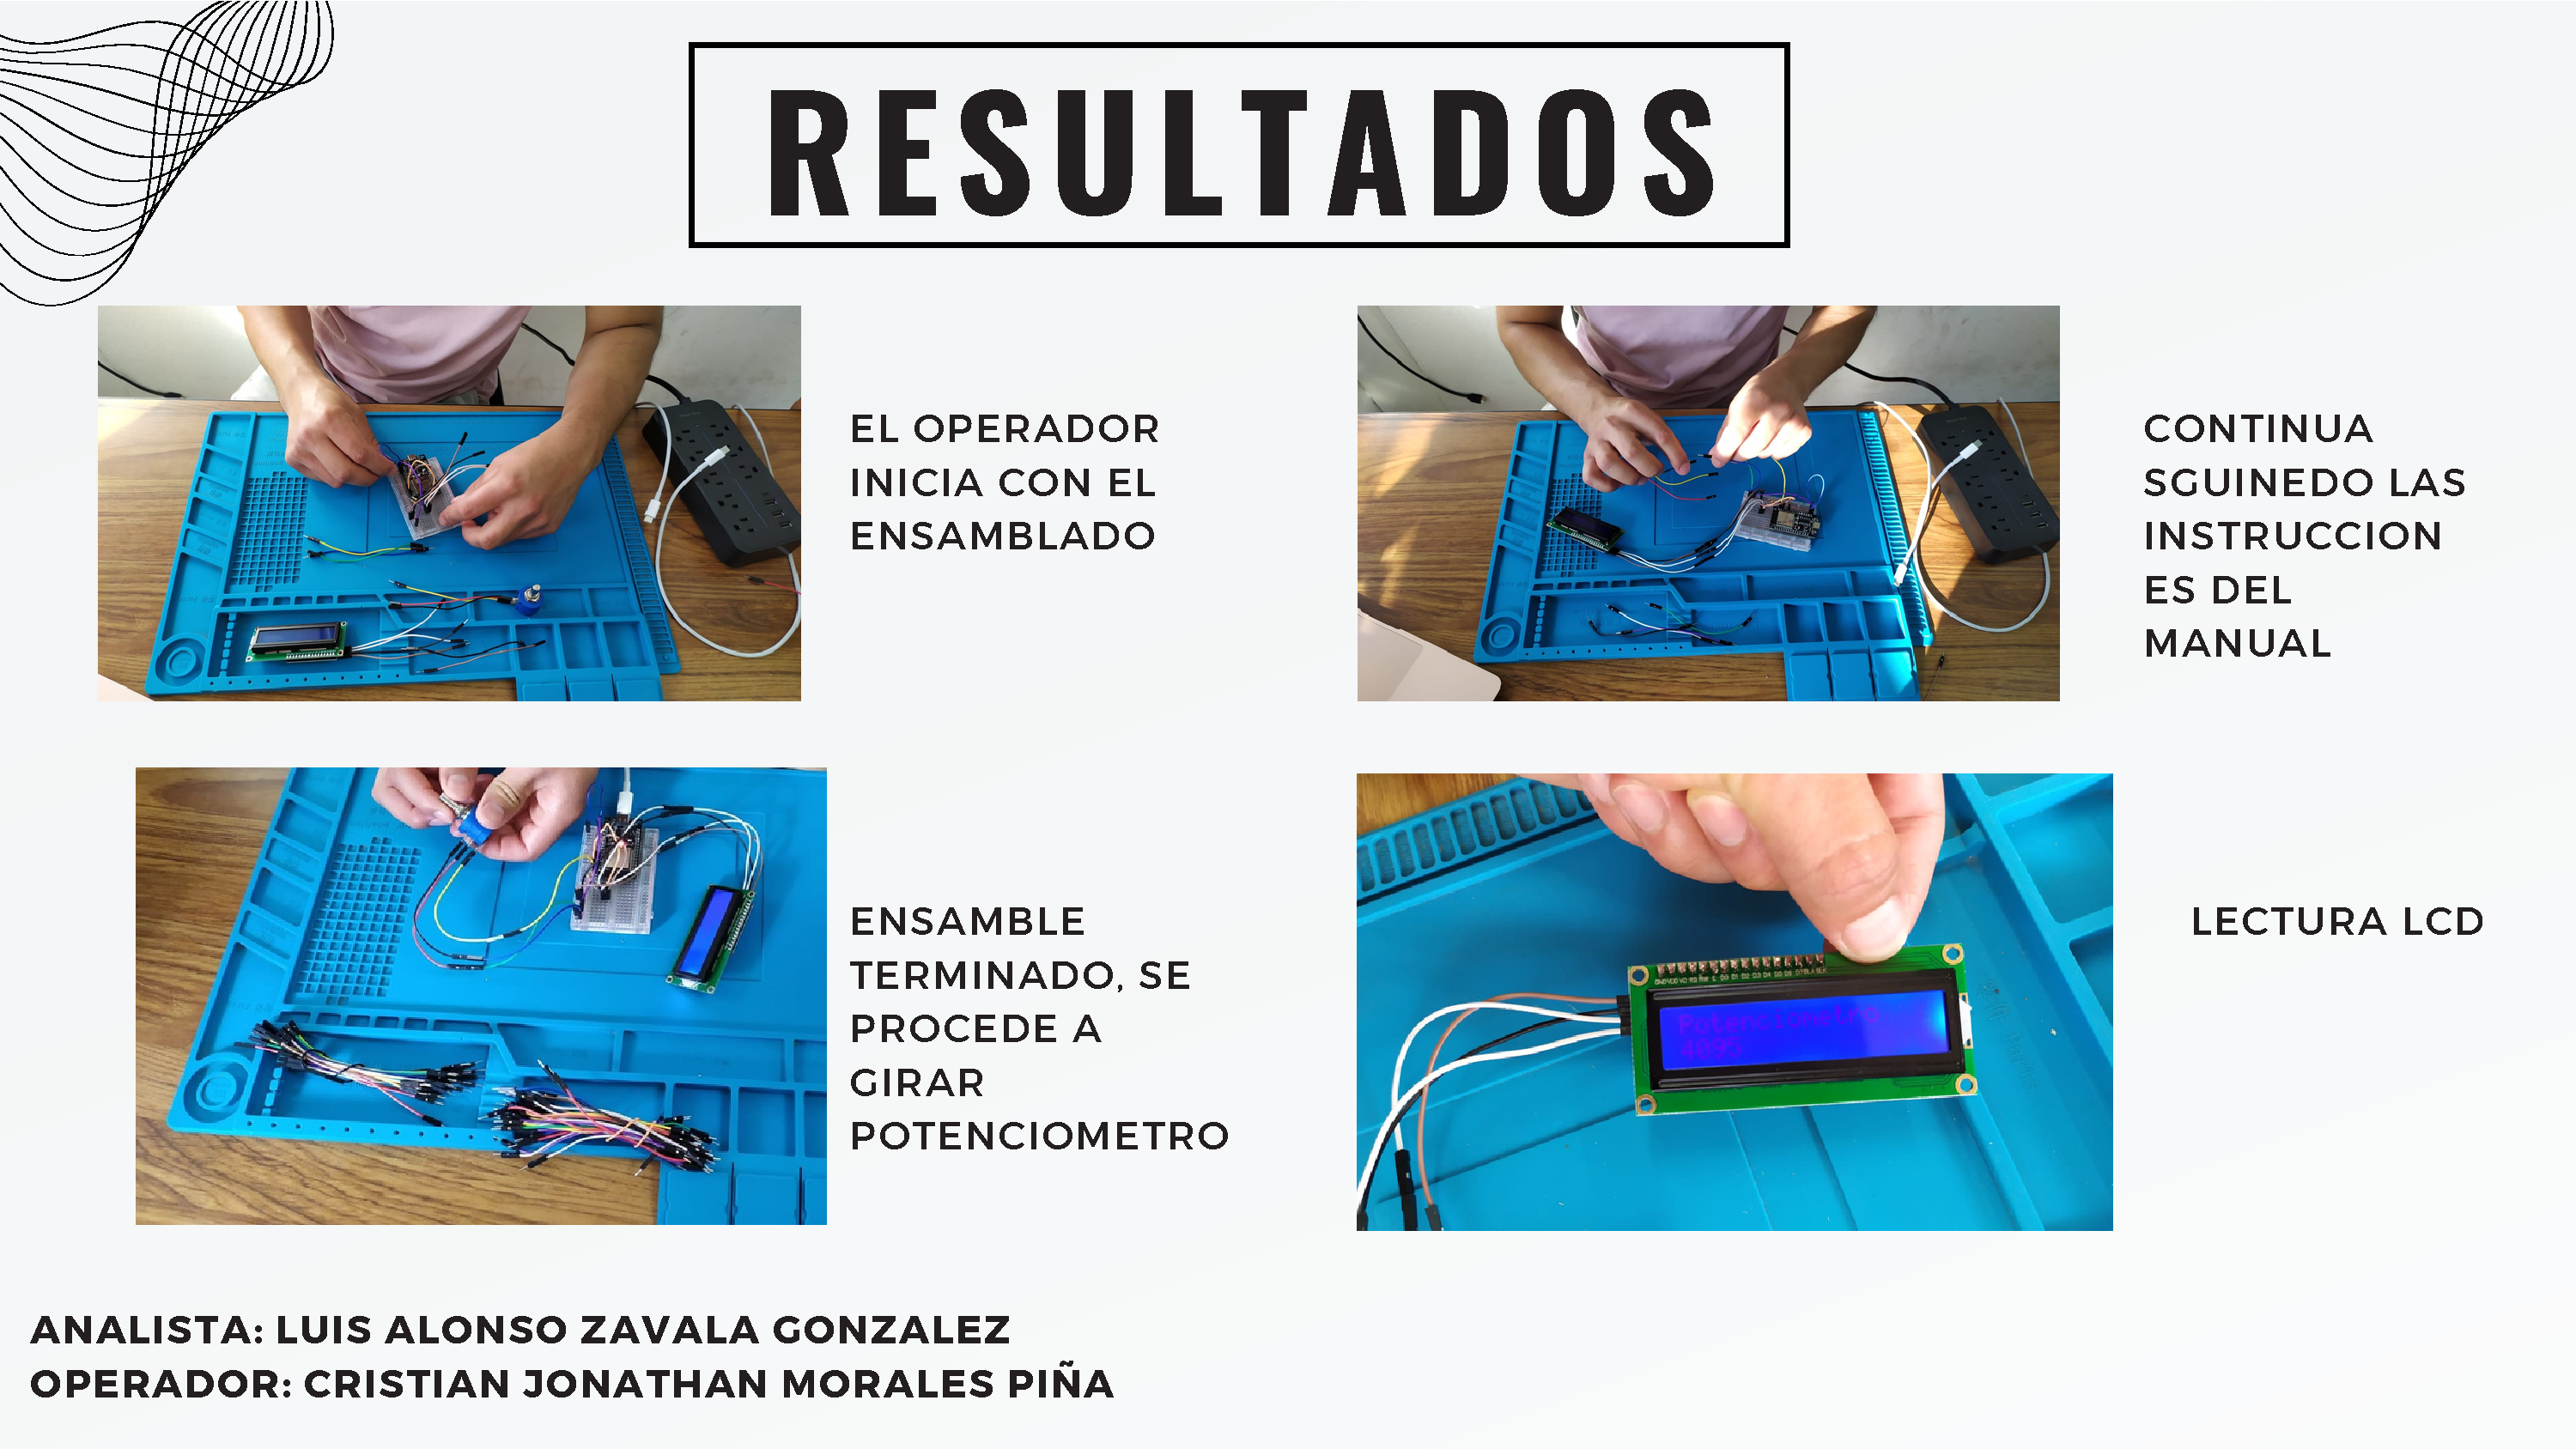
\includepdf[pages=-]{35/Img/resultados.pdf}
    
    % 
    \centering{\section[\appendixautorefname{}]{Apéndice}}\label{anexo:manual}
    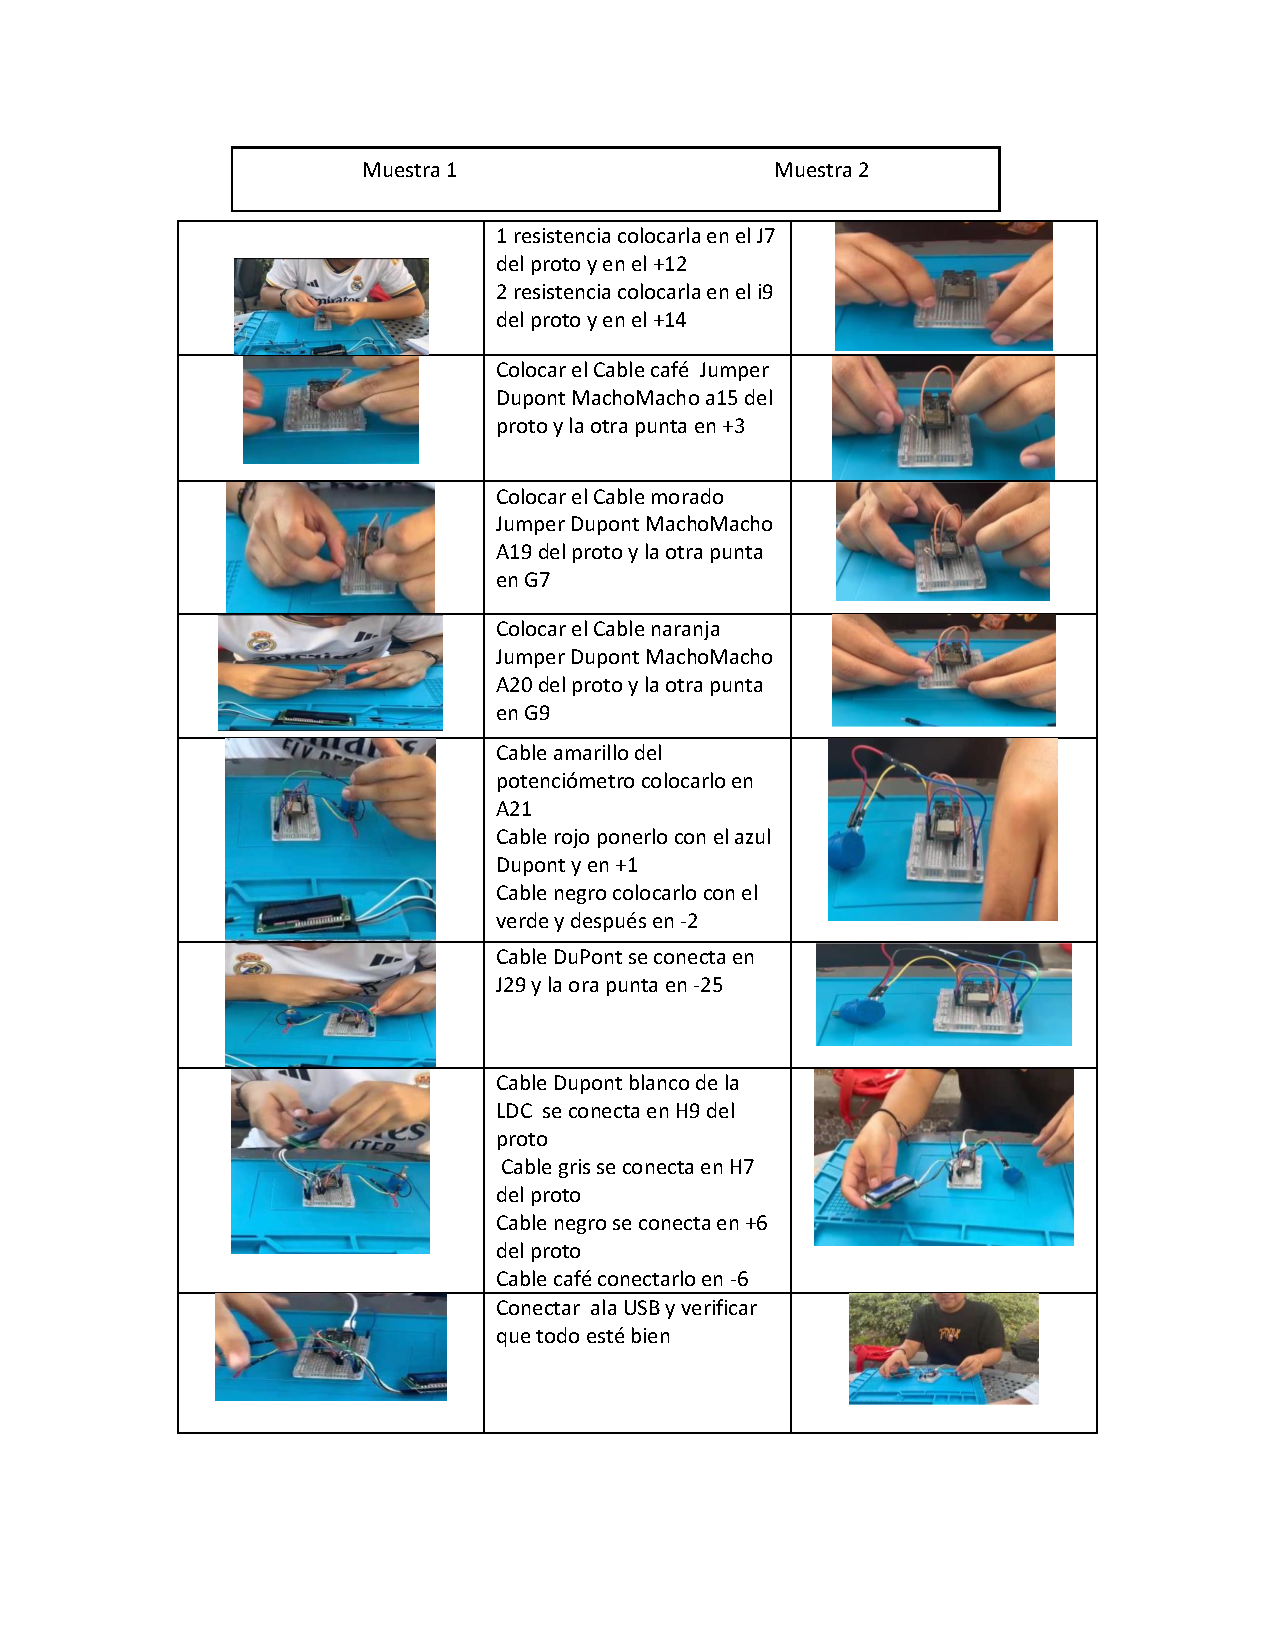
\includepdf[pages=-]{35/Img/manual.pdf}
    
    %
    \centering{\section[\appendixautorefname{}]{Apéndice}}\label{anexo:lcd}
    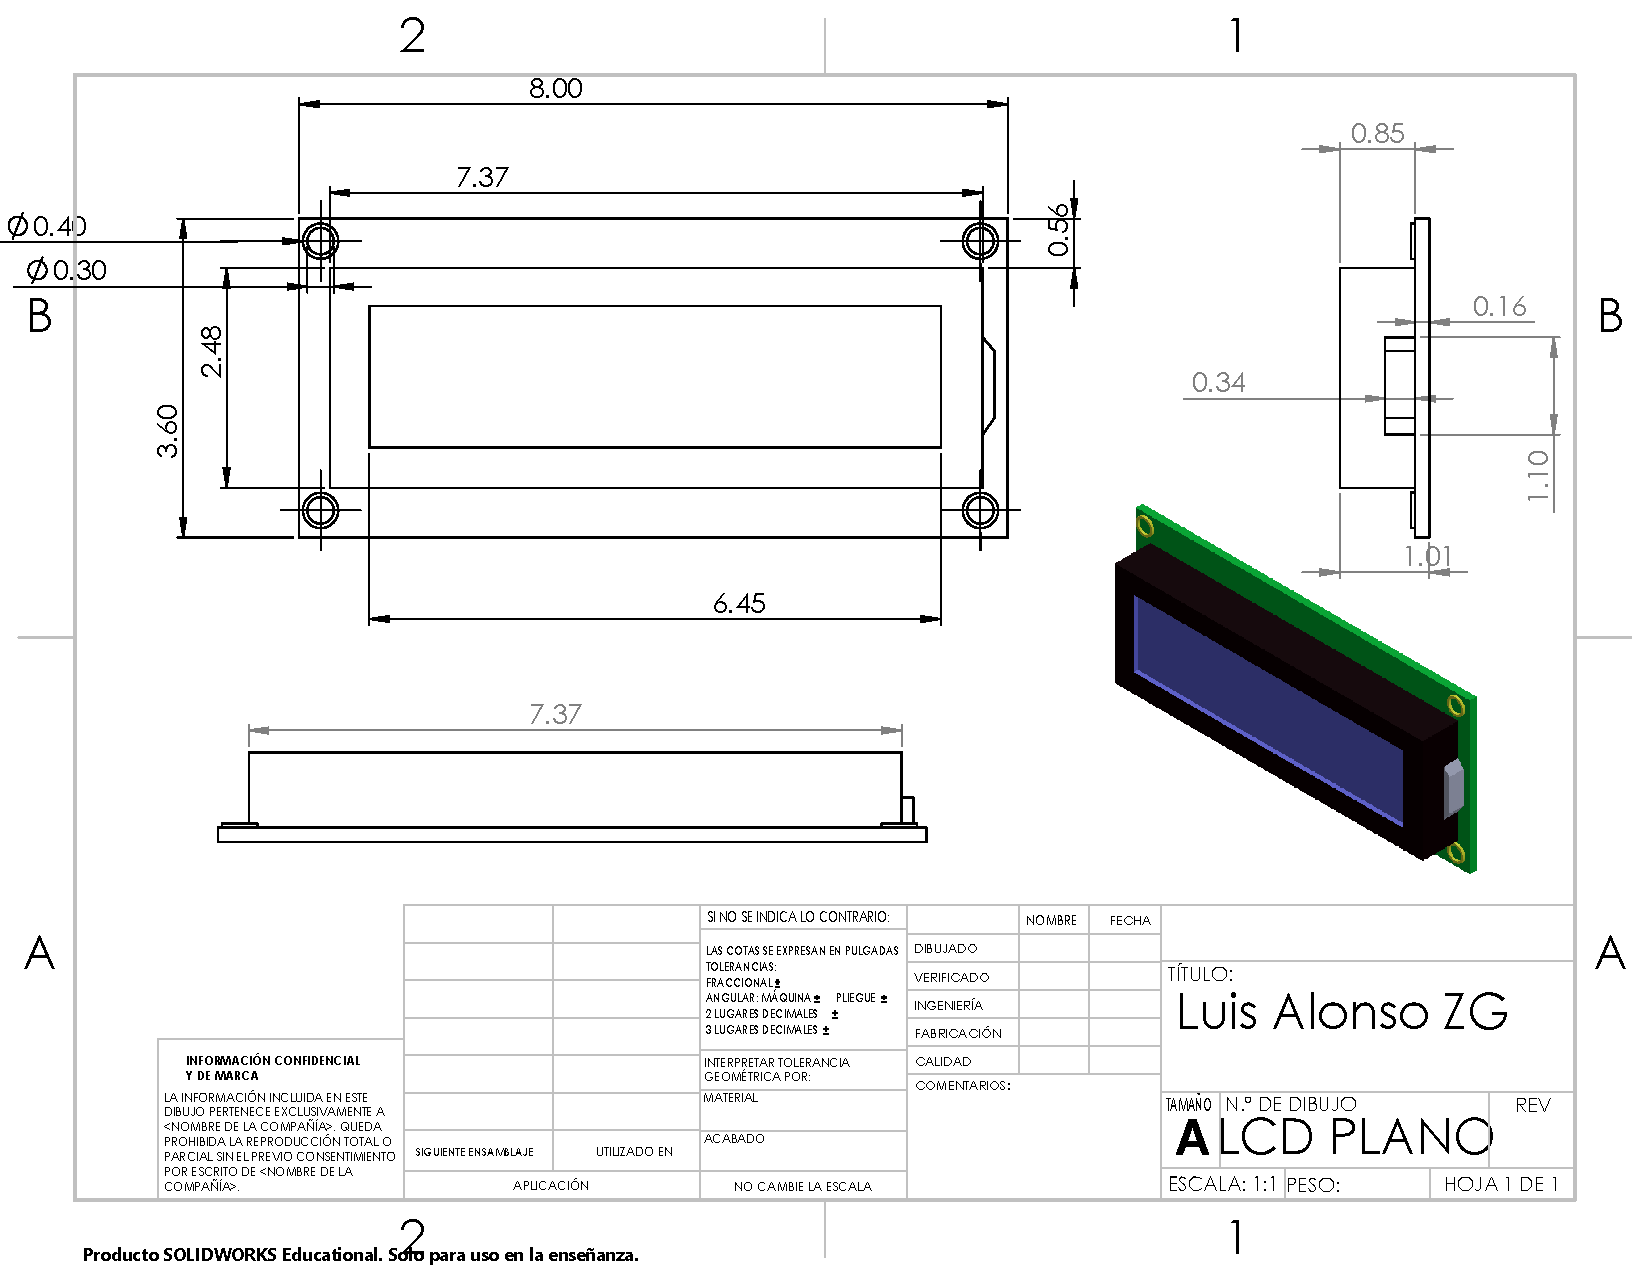
\includepdf[pages=-]{35/Img/lcdPlano.pdf}
    %
    \centering{\section[\appendixautorefname{}]{Apéndice}}\label{anexo:potenciometro}
    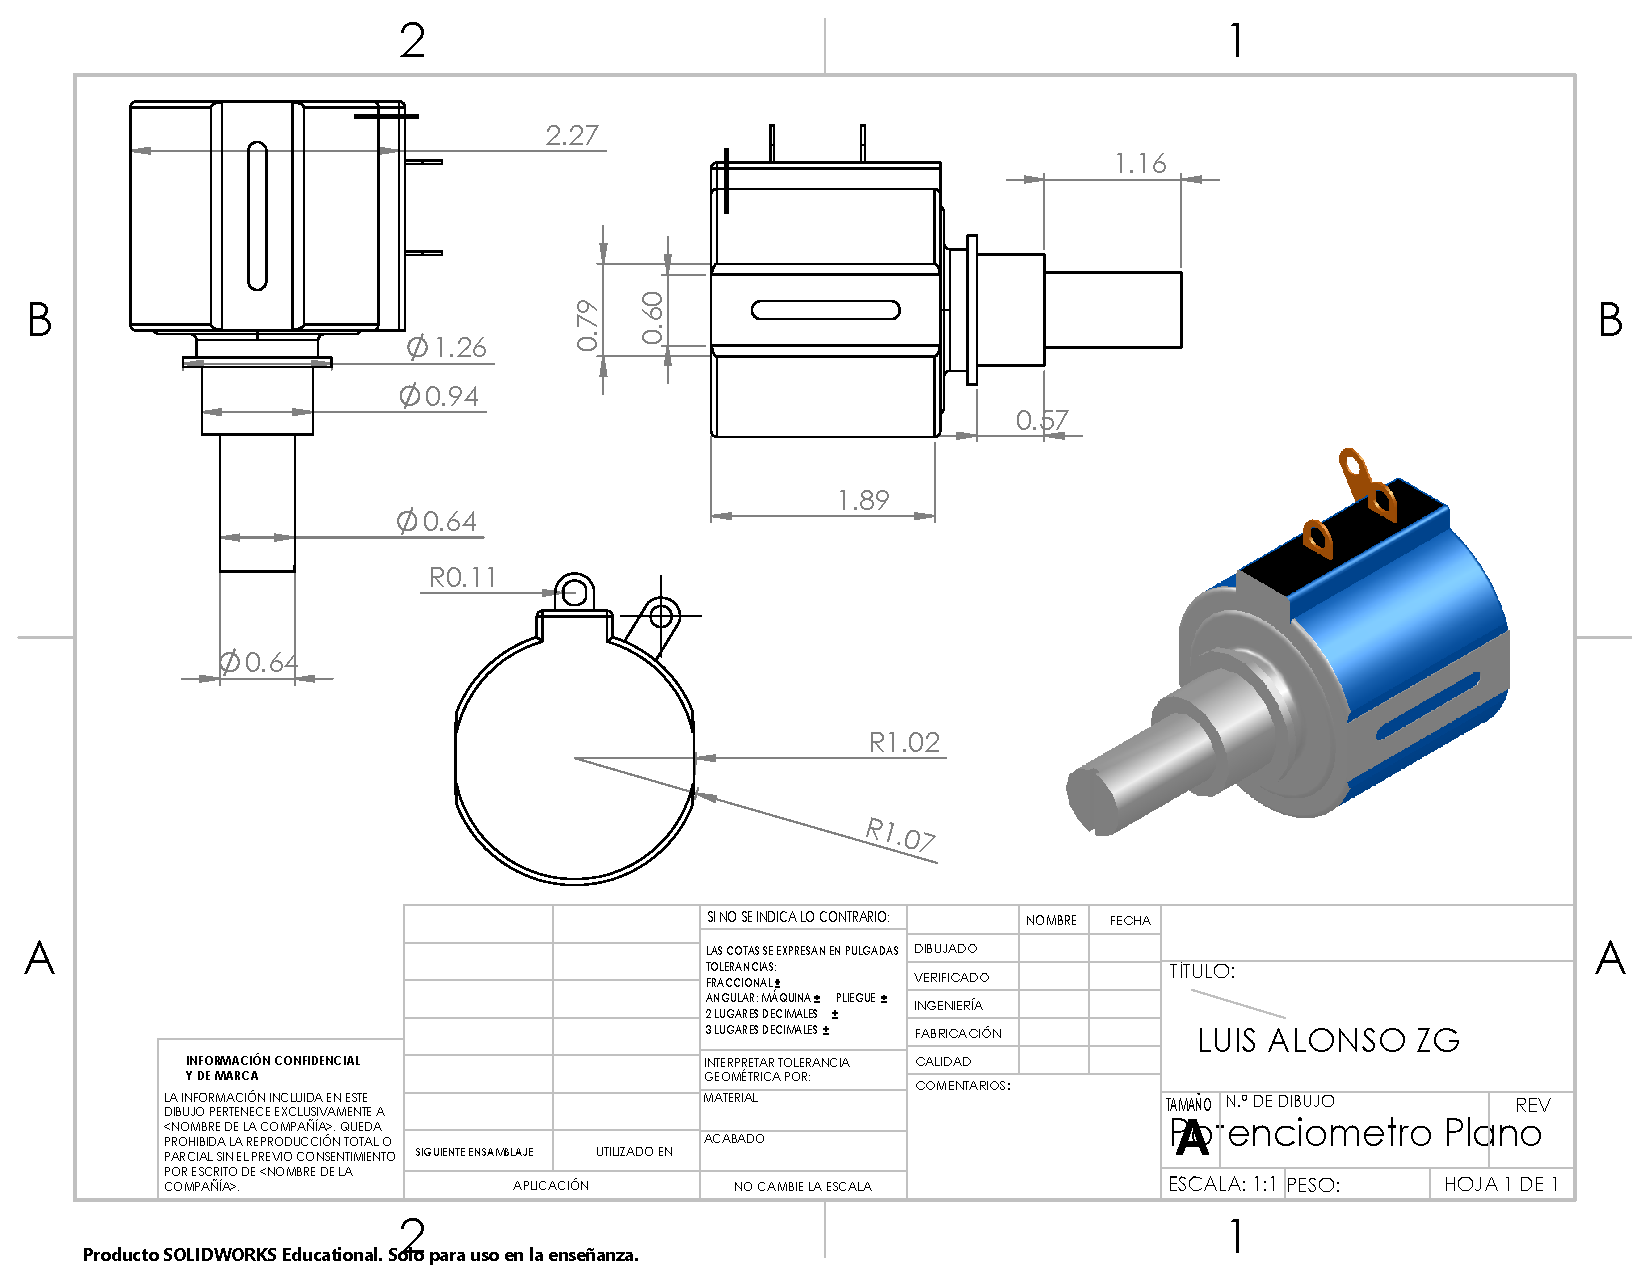
\includepdf[pages=-]{35/Img/potenciometroPlano.pdf}
    %
    \centering{\section[\appendixautorefname{}]{Apéndice}}\label{anexo:protoboard}
    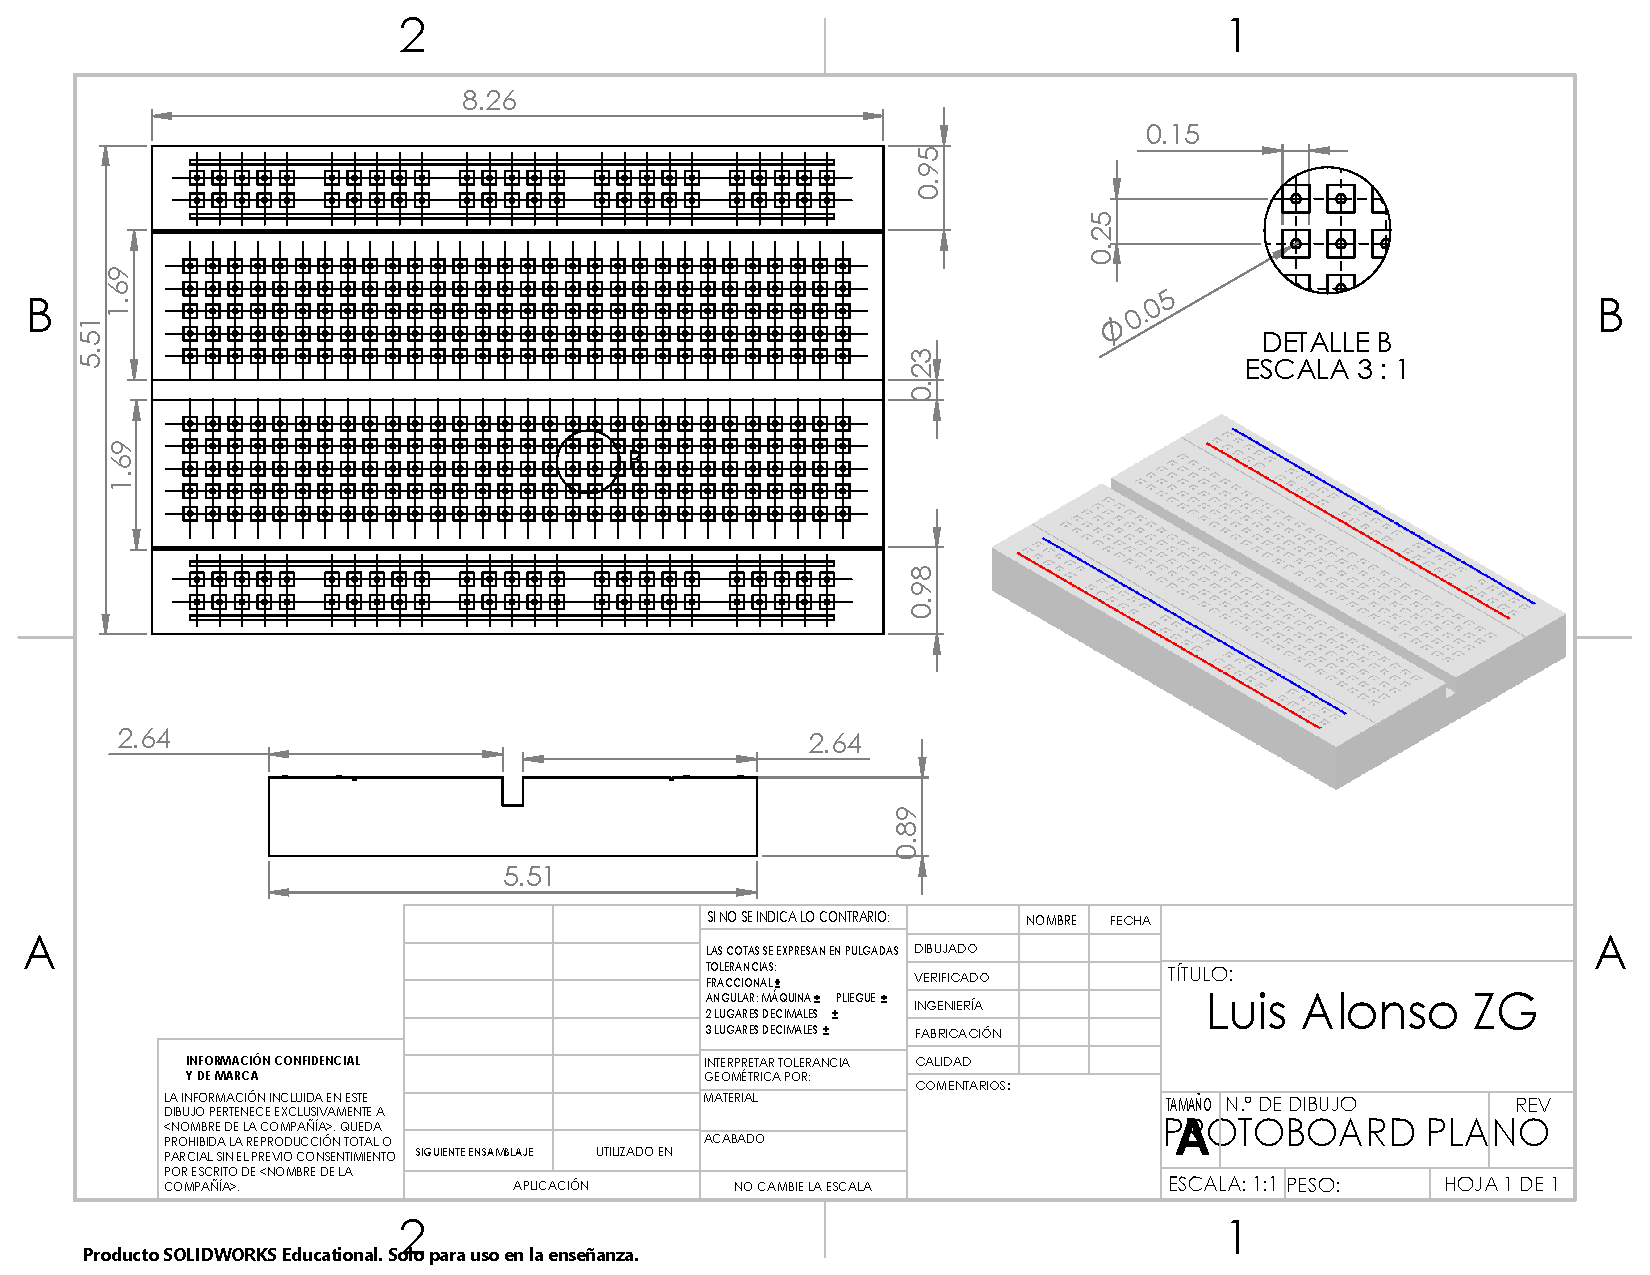
\includepdf[pages=-]{35/Img/protoboardPlano.pdf}
    %
    \centering{\section[\appendixautorefname{}]{Apéndice}}\label{anexo:resistencia}
    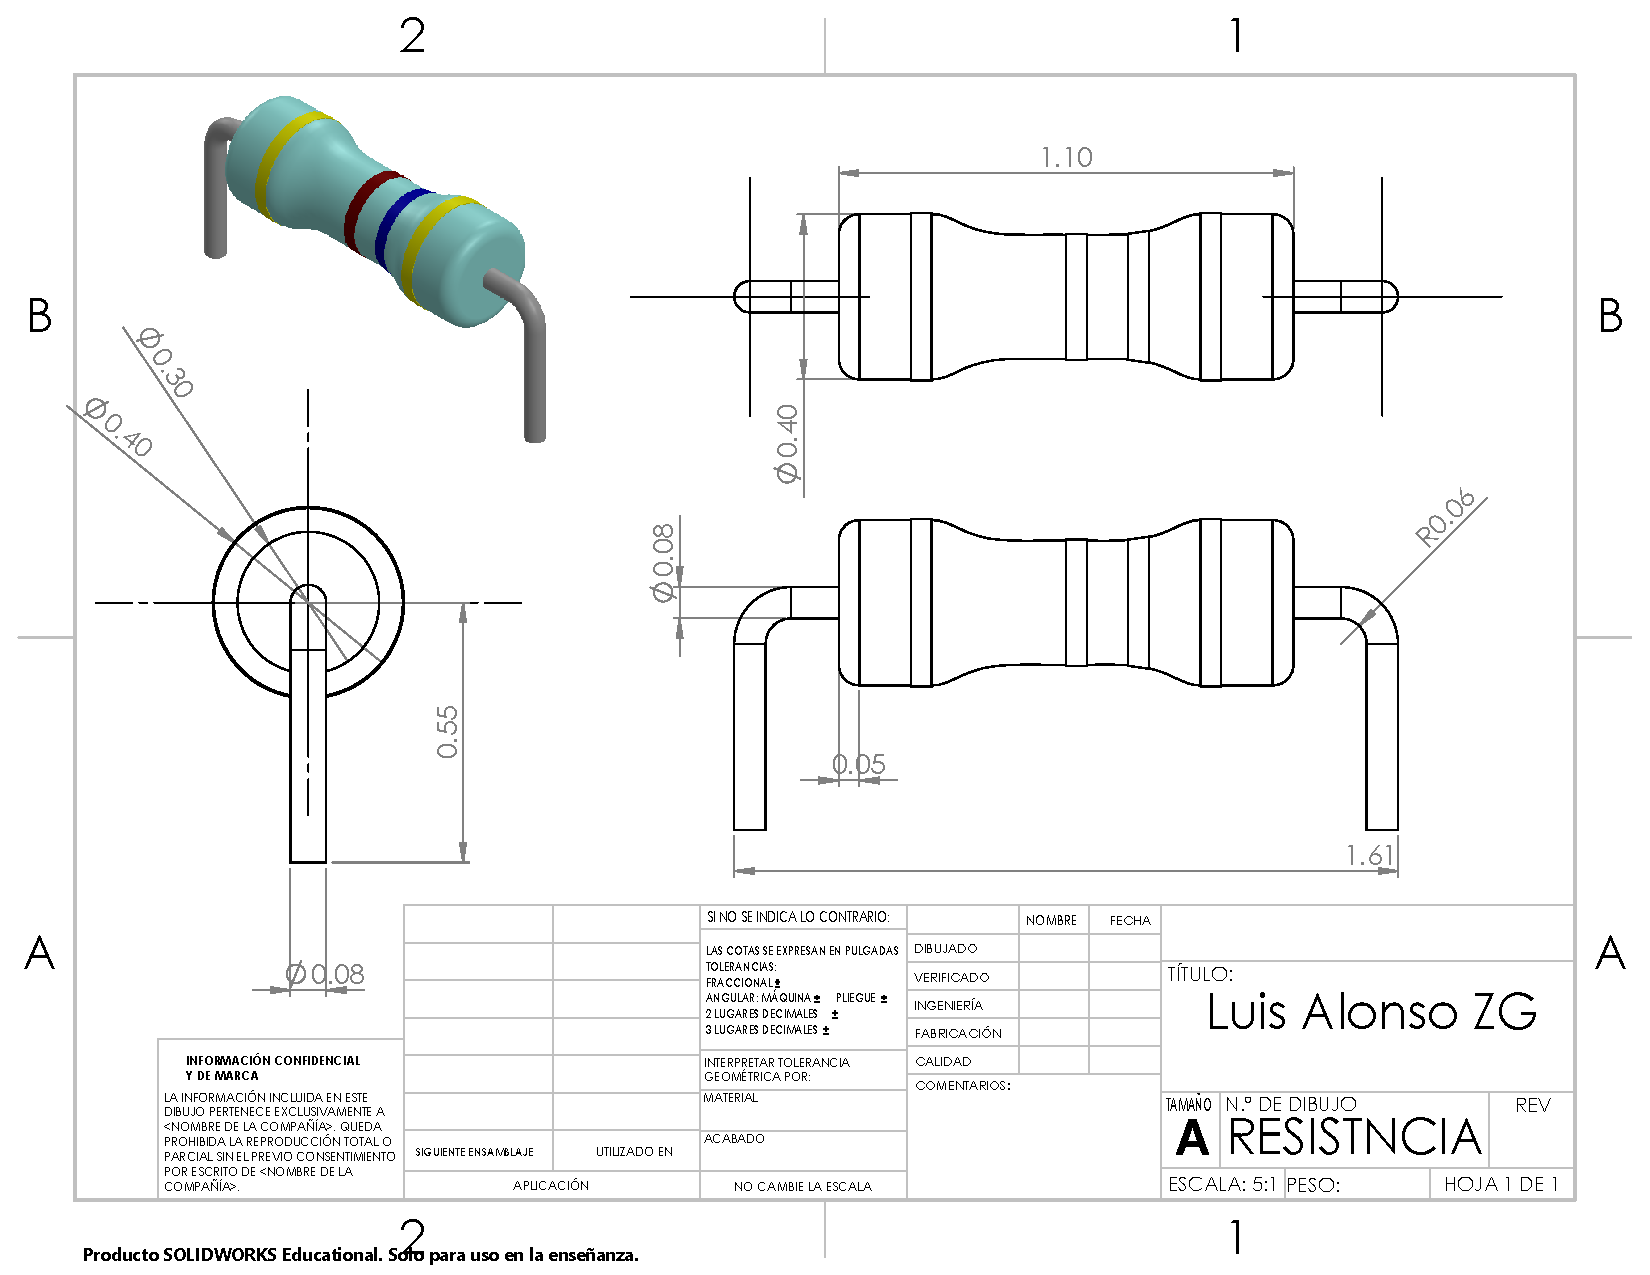
\includepdf[pages=-]{35/Img/resistenciaPlano.pdf}
    %
    \centering{\section[\appendixautorefname{}]{Apéndice}}\label{anexo:cableMH}
    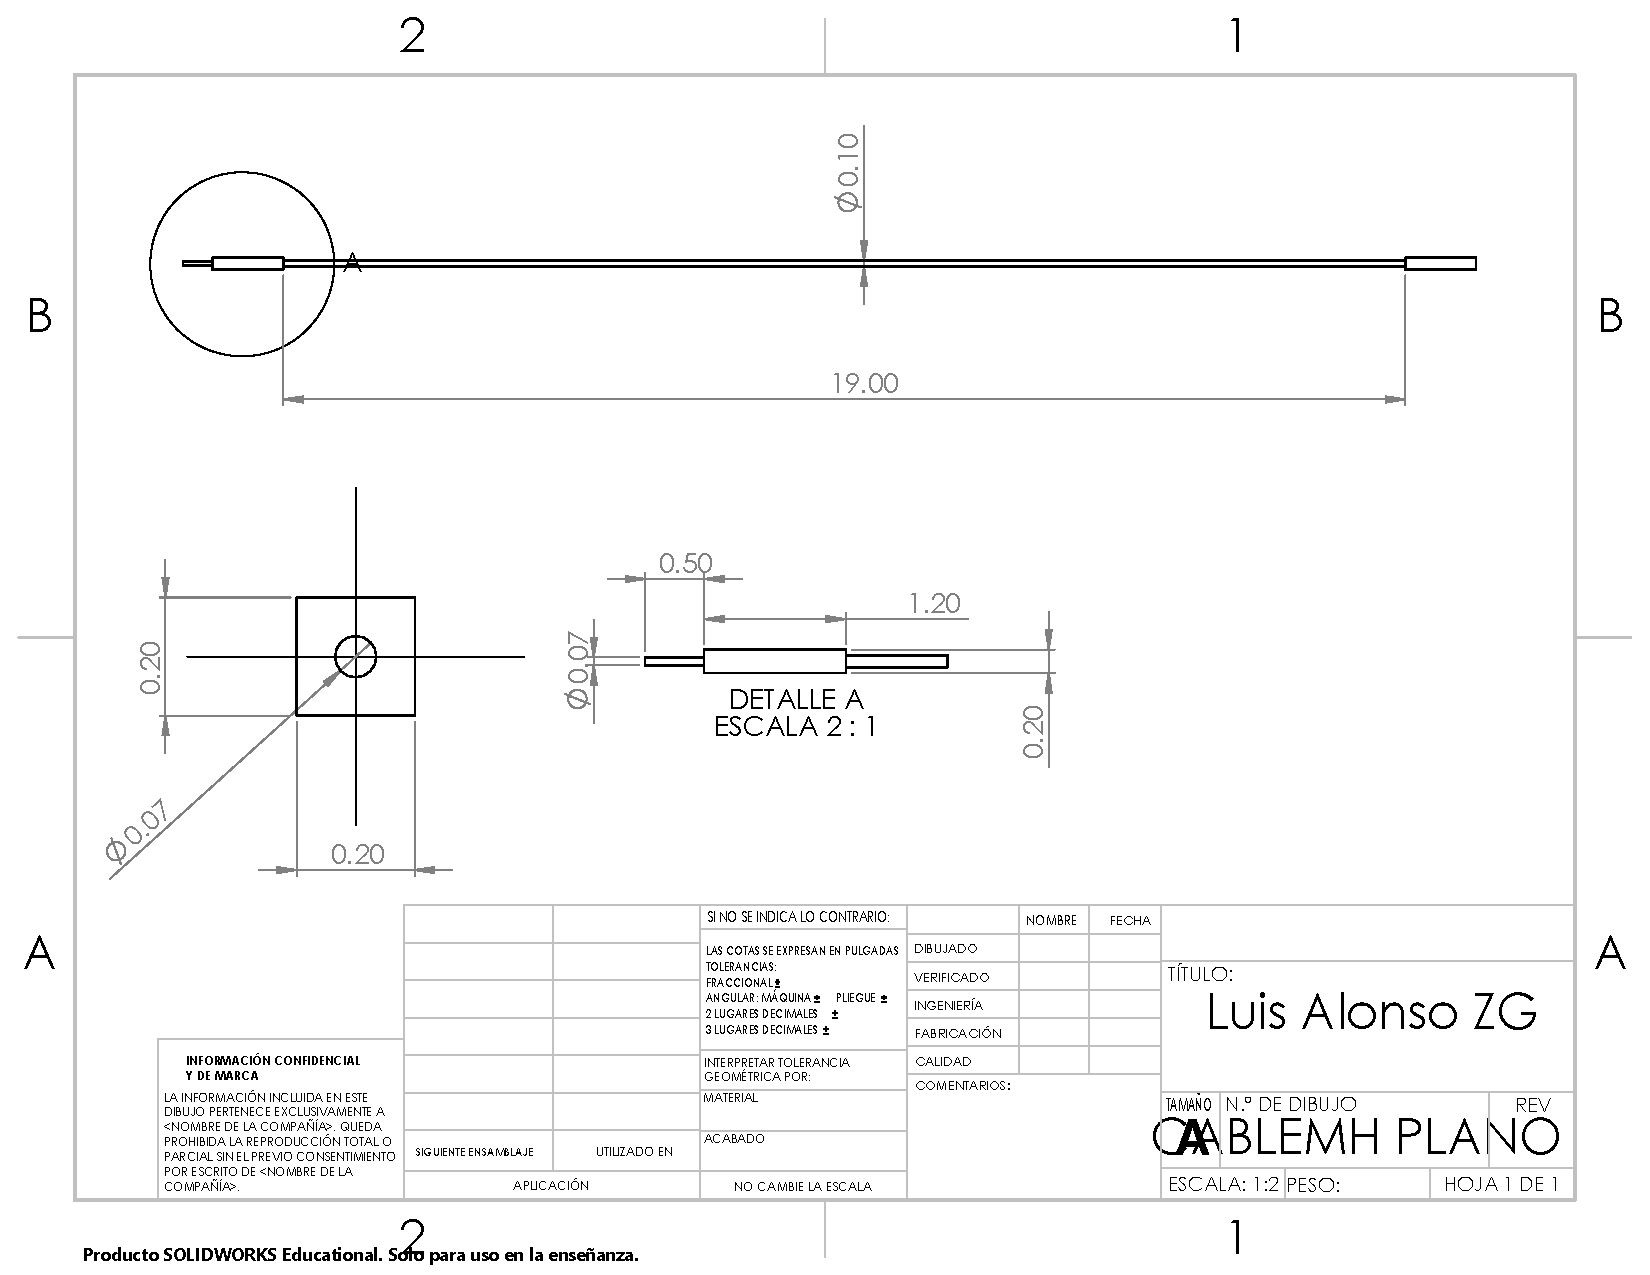
\includepdf[pages=-]{35/Img/cableMHPlano.pdf}
    %
    \centering{\section[\appendixautorefname{}]{Apéndice}}\label{anexo:cableMM}
    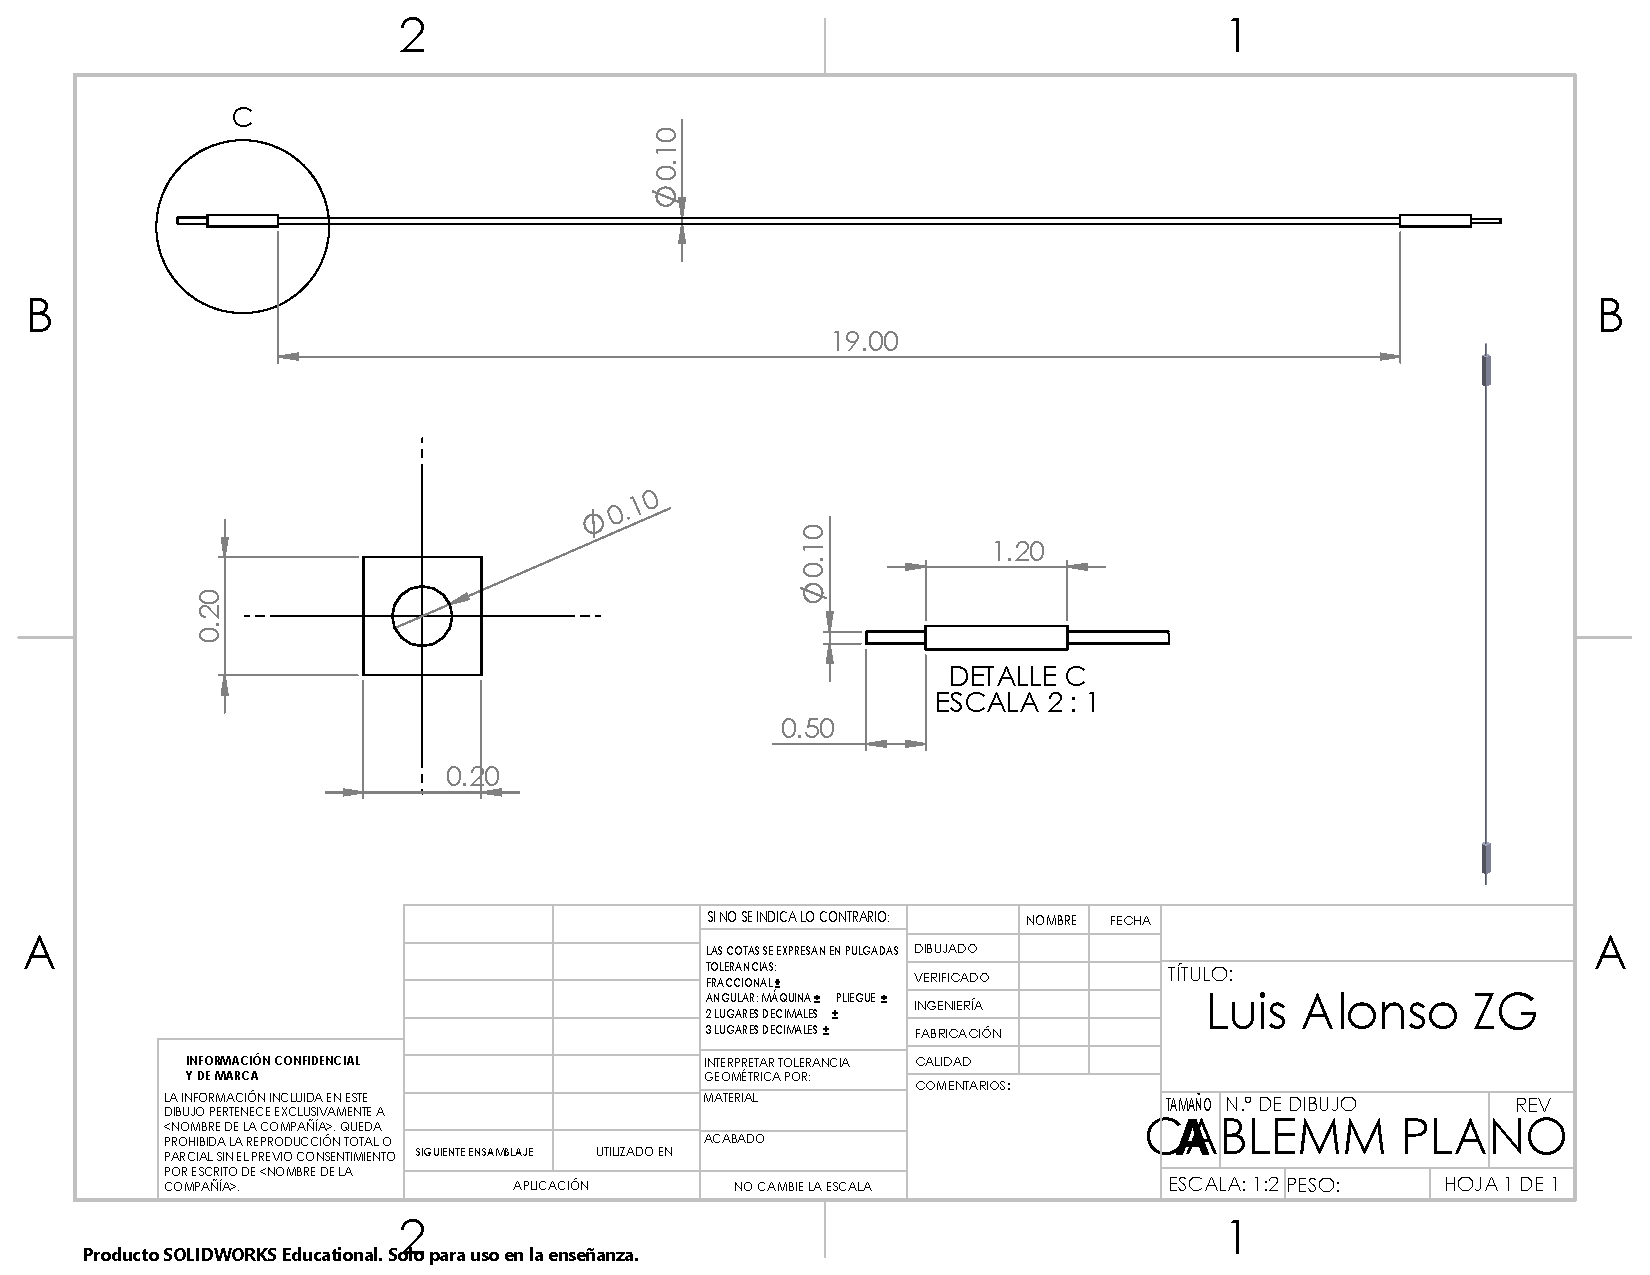
\includepdf[pages=-]{35/Img/cableMMPlano.pdf}
    %%%%%%%%%%%%%%%%%%%%%%%%%%%%%%%%%%%%%%%%